\clearpage
\subsection{Statistische Analyse von Graphit}
Wir werden uns nun eine Mikroskopieaufnahme des Graphits vornehmen und anhand dessen zeigen,
wie mithilfe der statistischen Analyse Gittereigenschaften extrahieren können. 
Die Vorliegende Aufnahme ist noch unbearbeitet
und dementsprechend schwierig zu analysieren (siehe Abbildung~\ref{fig:fourier1}).

\begin{figure}  
    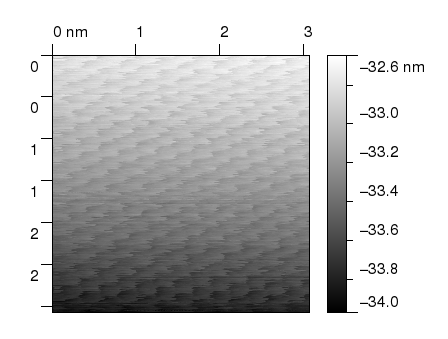
\includegraphics[width=10cm]{pics/fourier1}
  \caption{Unbearbeitete Aufnahme}
\label{fig:fourier1}
\end{figure}
\begin{figure}  
    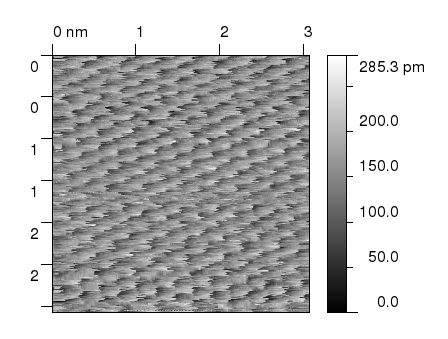
\includegraphics[width=10cm]{pics/fourier2}
  \caption{Aufnahme mit subtrahiertem Hintergrund.}
\label{fig:fourier2}
\end{figure}


Wir werden nun von mit einem lokalen Durchschnitt die Gradientenebene berechnen und diese
von der Mikroskopie subtrahieren (siehe Abbildung~\ref{fig:fourier2}). 
Abmessen von einer Reihe und Abzählen ergibt
\begin{align*}
    d_h &= 0.22 \pm 0.02 nm \mbox{ (horizontale Axe)}\\
    d_v &= 0.18 \pm 0.02 nm \mbox{ (vertikale Axe)}
\end{align*}


\begin{figure}  
    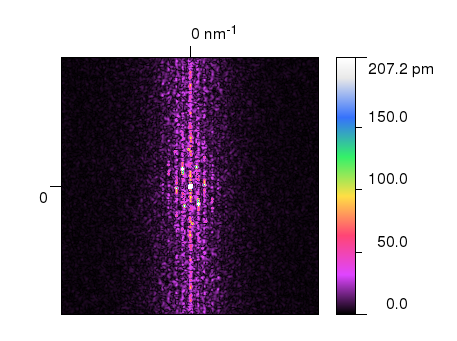
\includegraphics[width=10cm]{pics/fourier3}
  \caption{Modulus der 2DFFT (2-dimensionale Fast-Fourier-Transformation) 
      mithilfe der Blackman Windowfunktion
  der Aufnahme. Hier sieht man deutlich das vertikal verschobene Sechseck in der Mitte,
  welches die Moden der Aufnahme darstellt.}
\label{fig:fourier3}
\end{figure}

\begin{figure}  
    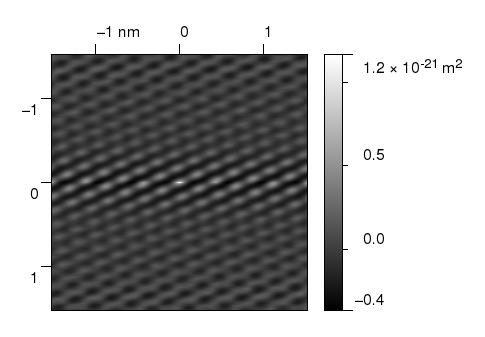
\includegraphics[width=8cm]{pics/fourier4}
    \caption{(Diskrete) Laplacetransformation (Kantenerkennung)
        von Abbildung~\ref{fig:fourier3}. Hier
    sind die Moden noch deutlicher zu sehen und können jetzt analysiert werden.}
\label{fig:fourier4}
\end{figure}
Wir sehen also, dass der vertikale Abstand, verglichen mit dem Literaturwert ($0.246nm$), deutlich
geringer ist, dass also die gesamte Aufnahme in diese Richtung zusammengezogen ist. 
Auch die horizontale Richtung ist im Mittel zu gering. Hierbei haben wir aber nur eine einzige
Linie analysiert, diese Methode ist allerdings sehr ungenau. 
Als nächstes können wir die Fouriertransformierte betrachten, dazu
berechnen wir die \textit{2DFFT} mithilfe der Windowfunktion \textit{Blackman} 
(siehe Abbildung~\ref{fig:fourier3}). Mithilfe einer Kantenerkennung können nun die Moden
abgelesen werden (in $nm^{-1}$ mit einer Ungenauigkeit von $0.1nm^{-1}$):
\begin{equation}
 \left \{ 6.4, 4.5, 6.1, 6.4, 4.6 \right \} 
\end{equation}
Die erwartete Wellenzahl wäre $4.065 nm^{-1}$, somit sehen wir, dass die meisten
Wellenzahlen darüber liegen. Dies liegt daran, dass wie wir schon eben beobachtet haben, dass
in der Orginalaufnahme die Abstände im Mittel zu gering waren, somit ergibt sich dass die 
Wellenzahlen zu hoch sind.



\clearpage
